  % ---------------------------------------------------------------------------
  \section{Empirical Diagnostics}
  \label{sec:empirical}
  % ---------------------------------------------------------------------------

  The real-system experiments do not expose an independent state-only witness
  $W_t$ for $S_t$. They therefore report a topology-derived capacity map with
  min-cut value $\varepsilon_\text{state}^\text{UB}$, and an action-relevance
  lower certificate $\delta_\text{act}^\text{LB}$. By
  Corollary~\ref{cor:action-mediated-unrec}, every positive
  $\delta_\text{act}^\text{LB}$ is also an action-mediated lower bound on
  $H(S_t\mid\tilde T_t)$. ReAct intervention and controlled replay
  (\S\ref{sec:exp-intervention}) show the same unlogged scratchpad dormant on
  calculator tasks and active on planning tasks. The LLaDA and multi-agent
  probes index $\Delta(j)$ by denoising step and peer-report edge, respectively
  (\S\ref{sec:diffusion-dynamic}--\ref{sec:multi-agent-private-report}).
  Independent state-witness calibration is provided by the synthetic
  ground-truth experiment in Appendix~\ref{app:synthetic}. All pipelines run on
  a single M4 Max workstation.

  \subsection{Capacity Map: Min-Cut and Logging Ablation}
  \label{sec:exp-static} 

  We extract the time-unrolled DAG from Qwen2.5-7B-Instruct ReAct execution
  traces on tool-selection tasks (Fig.~\ref{fig:static}, left). Per-edge budgets
   $c_e$ are assigned from interface specifications (\S\ref{sec:static-cert});
  the min-cut on unlogged edges gives $\varepsilon_\text{state}^\text{UB}$.
  Varying logging levels recomputes the min-cut; Table~\ref{tab:static-results}
  reports the stepwise reduction from $16{,}464$ to $0$ bits. The dominant
  bottleneck is the scratchpad-read path ($16{,}384$ bits). The same structural
  computation also supplies the coordinate system for the diffusion-LM and
  multi-agent dynamic checks that follow.

  \begin{table}[t]
  \centering
  \begin{tabularx}{\columnwidth}{l l X}
  \toprule
  Logging level & $\varepsilon_\text{state}^\text{UB}$ (bits) & Bottleneck \\
  \midrule
  ReAct, output only & $16{,}464$ & scratchpad\_read $(16384)$ + router\_logits
  $(80)$ \\
  ReAct, +log router & $16{,}384$ & scratchpad\_read $(16384)$ \\
  ReAct, +log scratchpad & $0$ & none \\
  ReAct, full instrumentation & $0$ & none \\
  \midrule
  LLaDA-8B-Instruct ($K{=}128$) & $32{,}768$ & denoising interface \\
  Multi-agent, all logged & $0$ & none \\
  Multi-agent, peer report unlogged & $32{,}768$ & peer\_report $\to S_t$ \\
  \bottomrule
  \end{tabularx}
  \caption{Capacity-map geometry. Adding ReAct logs monotonically removes
  residual cut capacity; the same min-cut analysis localizes capacity in a
  scratchpad module, denoising interface, or peer-report edge. The LLaDA bound
  is independent of $K$ because repeated reuse of the same bounded latent
  interface does not increase the one-step information bottleneck.}
  \label{tab:static-results}
  \end{table}

  \begin{figure}[t]
  \centering
  
\includegraphics[width=0.48\textwidth]{figures/react_dag.pdf}
  \hfill
  
\includegraphics[width=0.48\textwidth]{figures/logging_ablation.pdf}
  \caption{Left: Time-unrolled DAG extracted from Qwen2.5-7B-Instruct ReAct
  execution (logical edges omitted for clarity). Red edges are unlogged. Dashed
  edges form the min-cut. Right: Logging ablation curve. Adding instrumentation
  at the bottleneck drops $\varepsilon_\text{state}^\text{UB}$ stepwise to
  zero.}
  \label{fig:static}
  \end{figure}

  These cuts put the later dynamic probes on a common map: a scratchpad module
  in ReAct, a denoising interface in LLaDA, and a peer-state edge in the
  multi-agent system.

  \subsection{Dynamic Causal Certificates: Intervention and Controlled Replay}
  \label{sec:exp-intervention}

  We separate the two axes with a dormant/active task split under one topology.
  The unlogged scratchpad is present in both cases: irrelevant for calculator
  tasks, necessary for planning tasks. Intervention perturbs the scratchpad
  (masking or replacement); controlled replay removes it entirely while holding
  $\tilde T_t$ fixed. Table~\ref{tab:intervention-results} reports JS divergence
   over realized tool actions. Table~\ref{tab:replay-results} reports JS
  divergence over the model's soft tool-token probability distribution; for the
  policy-readout replay contrast, the argmax tool counts are unchanged, so the
  evidence is a policy-probability shift rather than a realized-tool flip. Both
  action-relevance certificates are zero on dormant tasks and positive on active
  tasks. The topology, and therefore the capacity-map value
  $\varepsilon_\text{state}^\text{UB}$, is unchanged.

  \begin{table}[t]
\centering
\small
\begin{tabular}{llcc}
\toprule
Task & Perturbation & JS (bits; nats) & 95\% CI (bits) \\
\midrule
Calculator (dormant) & mask $0.7$ & $0.0000$; $0.0000$ & $[0,0]$ \\
Planning (active) & mask $0.7$ & $0.0188$; $0.0131$ & $[0.0070,0.0381]$ \\
Calculator (dormant) & replace $1.0$ & $0.0000$; $0.0000$ & $[0,0]$ \\
Planning (active) & replace $1.0$ & $0.0080$; $0.0056$ & $[0.0027,0.0167]$ \\
\bottomrule
\end{tabular}
\caption[Intervention contrast by perturbation.]{Dynamic intervention contrast under
fixed ReAct topology. Dormant calculator rows are near zero, while active
planning rows are positive.}
\label{tab:intervention-results}
\end{table}


  The pair of tables isolates the transition from high structural capacity with
  zero action-mediated lower certificate to high structural capacity with
  positive action-mediated lower certificate: the hidden channel is structurally
  present in both task splits, but it becomes action-relevant only on planning
  tasks.

  \begin{table}[t]
\centering
\small
\begin{tabular}{llccc}
\toprule
Task & Replay & JS (bits; nats) & 95\% CI & Argmax \\
\midrule
Calc. (dormant) & removed & $0.0000$; $0.0000$ & $[0,0]$ & same \\
Planning (active) & removed & $0.0163$; $0.0113$ & $[0.0124,0.0208]$ & same \\
\bottomrule
\end{tabular}
\caption[Soft-policy replay contrast.]{Soft-policy replay contrast under fixed
topology. Wild episodes keep the full hidden scratchpad; replay episodes use the
same visible trace but remove the hidden scratchpad.}
\label{tab:replay-results}
\end{table}


  Under this fixed topology, the unlogged scratchpad contributes $16{,}384$ bits
   to $\varepsilon_\text{state}^\text{UB}$ in both task splits, matching the
  min-cut from the extracted ReAct DAG. Intervention and replay are zero on
  calculator tasks and positive on planning tasks. The capacity-map value is set
  by the deployment boundary and logging policy; residual decision relevance
  depends on which hidden channels the task uses. The positive planning rows are
  also action-mediated non-recoverability certificates by
  Corollary~\ref{cor:action-mediated-unrec}; they are not independent
  state-only witness certificates. The controlled replay row should be read as
  a pre-sampling policy-readout certificate, not as a realized-action flip.

  \subsection{Temporal Certificate Analysis on a Diffusion LM}
  \label{sec:diffusion-dynamic}

  ReAct gives a module-level contrast: the scratchpad is either used or not
  used. A diffusion LM gives a temporal contrast. The hidden channel exists
  throughout the $K$-step denoising trajectory, but its decision relevance need
  not be constant across steps.

  We use LLaDA-8B-Instruct with $K{=}10$ denoising steps on tool-selection
  prompts. A Gaussian perturbation ($\sigma{=}5.0$) is applied to layer-1
  activations at steps $\{2,4,6,8,10\}$; a late-layer perturbation is tracked as
   a broad sensitivity control. Each point uses $n{=}20$ trajectories and a
  trajectory-block bootstrap with $1{,}000$ resamples.

\begin{figure}[t]
\centering
\small
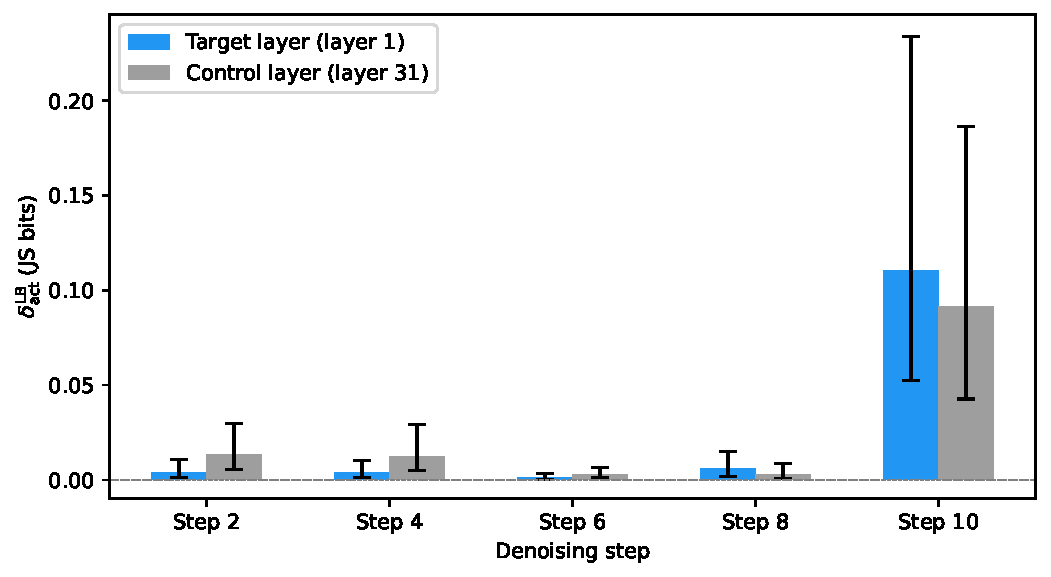
\includegraphics[width=0.62\textwidth]{figures/llada_temporal.pdf}
\caption{Temporal activation profile for LLaDA-8B-Instruct. Early denoising
steps are low, while step 10 has much larger target and control-layer
certificates, indicating late-binding decision relevance.}
\label{fig:llada-temporal}
\end{figure}

  The pattern is late-binding. Steps 2--8 remain near the floor for the target
  layer ($0.001$--$0.006$ bits), while step~10 rises to $\LladaFinalBits$ bits
  with 95\% CI $\LladaFinalCI$. The control layer also rises at step~10
  ($\LladaControlFinalBits$ bits, CI $\LladaControlFinalCI$), so the sensitivity
  is global rather than confined to the chosen layer. LLaDA carries hidden
  capacity throughout denoising; it becomes action-relevant when the denoising
  state binds to a discrete tool choice.
  The step-10 value is therefore an action-mediated non-recoverability lower
  certificate, not a direct entropy estimate of the full denoising latent.

  \subsection{Multi-Agent Private-Report Intervention}
  \label{sec:multi-agent-private-report}

  The multi-agent setting changes the index again. Here the controller delegates
   evidence gathering to a worker, so the worker's private report is not an
  auxiliary scratchpad but an epistemic edge in the decision graph. The worker
  sees a benchmark item and writes a short report; the controller sees only that
   report and chooses one API from \{\texttt{calculator}, \texttt{search}\}. The
   task pool combines $200$ GSM8K arithmetic items~\citep{cobbe2021training} and
   $200$ HotpotQA multi-hop fact questions~\citep{yang2018hotpotqa} with seed
  $42$.

  The main intervention replaces the worker report with a report from the
  opposite task class while holding the controller protocol fixed. A neutral
  replay removes the report content, and a same-class shuffle replaces it with
  another report from the same task class. An oracle-tag condition directly
  names and flips the API label to measure the binary ceiling. For each task and
   condition, the controller is sampled $k{=}8$ times; labels are parsed as
  \{\texttt{calculator}, \texttt{search}, \texttt{invalid}\}; and
  $\mathrm{JS}(P_\text{base},P_\text{condition})$ is averaged with a task-block
  bootstrap.

  \begin{table}[t]
\centering
\begin{tabular}{lcc}
\toprule
Condition & $\delta_\text{act}^\text{LB}$ (JS bits) & 95\% CI (bits) \\
\midrule
Neutral replay & $0.358$ & $[0.324,\ 0.392]$ \\
Counterfactual evidence & $0.901$ & $[0.873,\ 0.928]$ \\
Same-class shuffle & $0.084$ & $[0.060,\ 0.109]$ \\
Oracle tag upper-bound & $1.000$ & $[1.000,\ 1.000]$ \\
\bottomrule
\end{tabular}
\caption{Topological activation profile for the multi-agent deployment.
Counterfactual evidence nearly saturates the binary action ceiling, while
same-class shuffling remains much smaller. Hidden communication is therefore
behaviorally active when the controller has delegated evidence gathering to
the worker.}
\label{tab:multi-agent-dynamic}
\end{table}


  The contrast is topological. In ReAct, the scratchpad matters only when the
  task needs it. In the multi-agent deployment, the controller's decision is
  routed through the private worker report, so the active site is the
  communication edge itself. Same-class variation is local, neutral removal is
  substantial, and counterfactual evidence reaches
  $\MultiAgentCounterfactualBits$ bits, close to the oracle ceiling. This is
  again an action-mediated lower certificate: it shows that transcript-omitted
  private report state remains decision-relevant, while the capacity map reports
  how much private edge capacity could be hidden.
